\chapter{Steamship}

\vspace{\baselineskip}

\begin{paracol}{2}

\vspace{-0.2cm}
\begin{enumerate}
    \item Grab the \pickup{Phoenix Down} by the world map
\end{enumerate}
\vspace{-0.2cm}

\switchcolumn
\begin{steproute}{Before the Menu}
    \insertStep{../Graphics/Steps/37. Steamship 1.jpg}
    \insertStep{../Graphics/Steps/38. Steamship 2.jpg}
\end{steproute}

\switchcolumn
\begin{menu}{After Activating the Far Right Level}
    \varwb
    \begin{itemMenu}
        \potionMenu \ally{Faris (twice)}
        \item \menuHl{Ensure Ice Rod is slot 1}
        \item[] 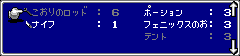
\includegraphics[scale=1.24]{../Graphics/Battle/3. Steamship Menu.png}
    \end{itemMenu}
    \begin{rowMenu}
        \swap Bartz \switch Galuf
    \end{rowMenu}
    \varwe
\end{menu}

\switchcolumn*
\begin{steproute}{Defeater x2 and CrewDust x2}
    \insertStep{../Graphics/Steps/39. Steamship Enc 1.jpg}
\end{steproute}

\switchcolumn
\begin{encounter}{Defeater x2 and CrewDust x2}
    \varwb
    \begin{notes}
        \item \encounterHl{Don't flee buffer}
        \item \encounterHl{You need to do inputs FAST}
    \end{notes}
    \begin{round}{1}
        \bartz Fight \then \ally{Galuf}
        \begin{notes}
            \item[] \encounterNote{(A)(\pointRight)(A)}
        \end{notes}
        \faris Defend
        \begin{notes}
            \item[] \encounterNote{(Hold R+A)}
        \end{notes}
        \lenna Item \then \battleGroup{Equip \iceRod} \then Break
        \begin{notes}
            \item[] \encounterNote{(\pointDown)(2A)(\pointUp)(3A)}
        \end{notes}
    \end{round}
    \varwe
\end{encounter}

\vspace{-0.25cm}
\begin{enumerate}[resume]
    \item Grab the \pickup{Elixir} before entering the boss room
\end{enumerate}
\vspace{-0.175cm}

\switchcolumn
\begin{steproute}{Before Liquid Flame}
    \insertStep{../Graphics/Steps/40. Steamship 3.jpg}
\end{steproute}

\switchcolumn
\begin{menu}{Before Liquid Flame}
    \varwb
    \begin{jobMenu}
        \lenna Time Mage \textbf{(\pointDown)} \optimize
        \faris Red Mage \textbf{(2\pointLeft)} \optimize
    \end{jobMenu}
    \begin{magicMenu}
        \faris \cure \space \then \ally{All to full}
    \end{magicMenu}
    \varwe
\end{menu}

\begin{boss}{Liquid Flame}
    \varwb
    \begin{round}{1}
        \bartz Item \then \battleGroup{Equip \knife} \then Defend
        \faris Item \then \battleGroup{\iceRod} \then Break
    \end{round}
    \begin{itemize}
        \item \newbox\hand \sbox\hand{\textbf{\ul{Round 2 (Hand)}}} \bossHl{{\usebox\hand}} 
        \begin{itemize}
            \lenna Defend
            \bartz Fight
            \faris
            \begin{itemize}
                \item \textit{If Lenna or Bartz died:} Item \then \battleGroup{\phoenixDown}
                \item \textit{Otherwise:} Item \then \battleGroup{Equip \iceRod } \then Break
            \end{itemize}
        \end{itemize}
    \end{itemize}
    \begin{itemize}
        \item \newbox\tornado \sbox\tornado{\textbf{\ul{Round 2 (Tornado)}}} \bossHl{{\usebox\tornado}} 
        \begin{itemize}
            \lenna Item \then \battleGroup{\iceRod} \then Break
        \end{itemize}
    \end{itemize}
    \varwe
\end{boss}

\end{paracol}